\section{A quick introduction to Topological Data Analysis}

TDA utilizes concepts from combinatorial, algebraic, and differential topology to investigate how data is shaped within its ambient space. It is standard to assume that data resides in, or is sampled from, underlying metric spaces and smooth manifolds. This assumption ensures that applications, such as triangulations, can faithfully represent the data and capture its intrinsic topological invariants.

A core technique in TDA is filtration, a concept rooted in combinatorial and algebraic topology. To construct connected and structured simplicial complexes, the filtration process generates a nested sequence of these complexes based on a proximity parameter that iteratively increases. Using this nested sequence, we can calculate the data's persistent homology. This framework is highly robust to noise \cite{cohen2005stability} and explicitly reveals when topological invariants (and, if in a Euclidean space, geometrical holes) appear and disappear as the simplicial complex evolves.

\begin{figure}[H]
    \centering 
    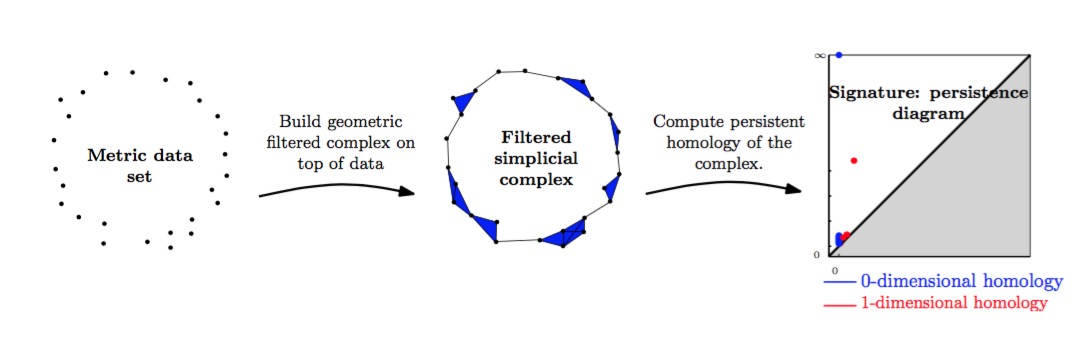
\includegraphics[width=1\linewidth]{imgs/Illustration_of_Typical_Workflow_in_TDA.jpeg}
    \caption{Illustration of a typical workflow in Topological Data Analysis}
    \label{fig:placeholder}
\end{figure}

When the true shape of the dataset is known, we can use the persistence diagram to find a proximity threshold $\varepsilon>0$ to construct a simplicial complex that faithfully emulates the geometry of the data.

% Side-by-side figures
\begin{figure}[H]
\centering
\begin{minipage}{.45\textwidth}
  \centering
  \includesvg[width=0.475\linewidth]{imgs/Simplicial_complex_example.svg}
  \captionof{figure}{Three dimensional Simplicial Complex, because its higher simplex has dimension 3, which is the tetrahedron.}
  \label{fig:test1}
\end{minipage}\hfill
\begin{minipage}{.45\textwidth}
  \centering
\includesvg[width=0.475\linewidth]{imgs/A_triangulation_of_the_torus,_with_bounding_box_fixed.svg}
  \captionof{figure}{A triangulation can be understood as a two dimensional Simplicial Complex, since its higher dimensional simplex are triangles. }
  \label{fig:test2}
\end{minipage}
\end{figure}